\pdfsuppresswarningpagegroup=1
\pdfminorversion=7
% StM3 Assessed Exercise
% Template by: Dr. Antonio Melro <antonio.melro@bristol.ac.uk>
% Private use only
% Last modification: 11/12/2018$
%~~~~~~~~~~~~~~~~~~~~~~~~~~~~~~~~~~~~~~~~~~~~~~~~~~~~~~~~~~~~~
% Document size & margin definitions
\documentclass[11pt,a4paper,oneside]{memoir}
%~~~~~~~~~~~~~~~~~~~~~~~~~~~~~~~~~~~~~~~~~~~~~~~~~~~~~~~~~~~~~
%\counterwithout{section}{chapter}
\setsecnumdepth{subsection}
\setsecnumdepth{subsubsection}
% Latex workpackages
\usepackage{amsmath}
\usepackage{amssymb}
\usepackage{graphicx}
\graphicspath{ {./figs/}}
\usepackage{mathpazo}
\usepackage{microtype} % Slightly tweak font spacing for aesthetics
\usepackage[pdfpagelabels]{hyperref}
\usepackage{booktabs}
\usepackage{multirow}
\usepackage{tikz}
\usepackage{xcolor}
\usepackage{framed}
\usepackage{geometry}
\newgeometry{innermargin=1.25in,top=1.25in,bottom=1in}
%\usepackage{caption}
\usepackage[tikz]{bclogo}
\usepackage{lipsum}
\hypersetup{
    colorlinks,
    citecolor=blue,
    filecolor=blue,
    linkcolor=blue,
    urlcolor=blue
}
%
\usepackage{textcase}
\newcommand{\theauthor}{\href{your.email@bristol.ac.uk}{Your name}}
\newcommand{\studentid}{ab12345}
\newcommand{\tutor}{\href{tutor.email@bristol.ac.uk}{Tutor name}}
\newcommand{\coursetitle}{Structures \& Materials 3}
\newcommand{\thetitle}{Metallic Wing Torque Box\\Assignment Report}
\newcommand{\subtitle}{\sffamily\textls[200]{\MakeTextUppercase{Stress Analysis using MSC Patran/Nastran}}\normalfont}
\newcommand{\department}{Department of Aerospace Engineering \vspace{0.35cm}\par University of Bristol}
%
\newcommand{\monthyear}{\ifcase\month\or January\or February\or March\or April\or May\or June\or July\or August\or September\or October\or November\or December\fi\space\number\year} % A command to print the current month and year


% Begin document
\begin{document}
\pagenumbering{Alph}
% Title page
%\frontmatter

\begingroup
\thispagestyle{empty}
\newgeometry{innermargin=1in,top=1.0in,bottom=1in}

\setlength{\parindent}{0pt}
%\begin{minipage}[b]{0.5\linewidth}
%\vfill\fontsize{14}{14}\selectfont\textit{\department} 
%\end{minipage}
%\hspace{0.5cm}
%\begin{minipage}[b]{0.45\linewidth}
%\hfill
\includegraphics[width=6.0cm]{UoB-logo-black.pdf}
%\end{minipage}
\begin{minipage}[b][2.0cm]{0.5\linewidth}
\vfill\fontsize{14}{14}\selectfont\textit{\department} 
\end{minipage}
\begin{minipage}[b][2.0cm]{0.45\linewidth}
\hfill
\includegraphics[width=6.0cm]{UoB-logo-black.pdf}
\end{minipage}

\vspace{1.75in}\fontsize{36}{54}\selectfont\coursetitle

\vspace{.75in}\fontsize{36}{54}\selectfont\thetitle

\vspace{0.125in}\fontsize{14}{14}\selectfont\subtitle
\vfill
\begin{minipage}{0.48\textwidth}
\fontsize{16}{24}\selectfont\textsc{Student:}

\fontsize{16}{24}\selectfont\textsc{Student Number:}

\fontsize{16}{24}\selectfont\textsc{Tutor(s):}

\fontsize{16}{24}\selectfont\textsc{Academic Year:}
\end{minipage}
\begin{minipage}{0.48\textwidth}
\fontsize{16}{24}\selectfont\textnormal{\theauthor}

\fontsize{16}{24}\selectfont\textnormal{\studentid}

\fontsize{16}{24}\selectfont\textnormal{\tutor}

\fontsize{16}{24}\selectfont\textnormal{2018-19}
\end{minipage}

\restoregeometry
\endgroup

% abstract page
\newpage
~\vfill
\thispagestyle{empty}
\setlength{\parindent}{0pt}
\setlength{\parskip}{\baselineskip}
\large Academic Year \the\year-19 \par
\large Structures \& Materials 3 (AENG31200) \par
\large Academic Lead(s): \, \href{giuliano.allegri@bristol.ac.uk}{Dr.~Giuliano Allegri}, \href{antonio.melro@bristol.ac.uk}{Dr.~Ant\'{o}nio Rui Melro} \par
\par Department of Aerospace Engineering\index{license}

\par\textit{University of Bristol, \monthyear}
\cleardoublepage

\frontmatter
% Frontpage:
\renewcommand{\abstractname}{Summary}
\begin{abstract}
	Summary should be written in simple language (avoiding core technical terms) clearly stating the objective of the analysis, main conclusions and recommendations. It is meant for managers, decision makers and team members involved in the project who either do not have sufficient time to go through the complete report or are not familiar with FEA terminology. 
\end{abstract}

\clearpage
\tableofcontents% automatically create table of contents at second Latex run
\newpage
\listoffigures
\listoftables
\clearpage % start new page

\mainmatter
\chapterstyle{reparticle}
\pagestyle{ruled}

\chapter{Format of technical report}

The final report will be submitted online via SAFE as a PDF, no hardcopy necessary!
A report template is available on Blackboard. You may use either Microsoft Word, or \LaTeX. Technical report should include:
	\begin{enumerate}
		\item \textbf{Title or front page of report:} The title of the project, a nice small figure of the component, a report number, date of submission, name of supervisor, name of analyst (student), student contact details and affiliation.
		\item \textbf{Summary (maximum 1 page) of the project:} A summary should be written in simple language (avoiding core technical terms) clearly stating the objective of the analysis, main conclusions and recommendations. It is meant for managers, decision makers and team members involved in the project who either do not have sufficient time to go through the complete report or are not familiar with FEA terminology.
		\item \textbf{Main body of work:}
		\begin{enumerate}
			\item Aims/Scope of project.
			\item Brief description of component, basic design details, functionality.
			\item Methodology or strategy of analysis.
			\item Mesh details (element types used, number of elements etc.), quality checks.
			\item Material and sectional properties.
			\item Boundary conditions details with separate figure corresponding to the appropriate load case.
			\item Tabular results and clear figures of appropriate load case.
		\end{enumerate}
		\item \textbf{Conclusion and future work}
	\end{enumerate}

Documentation and local data storage/backup of all relevant models and results are essential.  

\chapter{Introduction to StM3 Assignment}\label{chap:intro}
\section{Aims/Scope of project}
\begin{enumerate}
	\item Explain in a few paragraphs the motivation for carrying out this work. 
	\item Discuss relevance of 2nd year AVDASI2 course module.
\end{enumerate}
%
\begin{quote}
...the aim of this assignment is for you to broaden your FE skills and have practical experience tackling a \textbf{real-world exercise} by using an aerospace industry-standard, FE software package; MSC Patran/Nastran. A useful reference is a peer-reviewed journal paper by Ostegaard et al.~on the application of virtual testing of aircraft structures using non-linear finite element models \cite{ostergaard2011virtual}...

...to realise this goal, a finite element model of a wing torque box is developed based on a generic design from AVDASI 2, see Fig.~\ref{fig:ASD2-DBT-Wing-5-revised}, and perform a linear static stress analysis to assess its structural performance (by calculating deflections and stresses)...
\end{quote}

\begin{figure}
  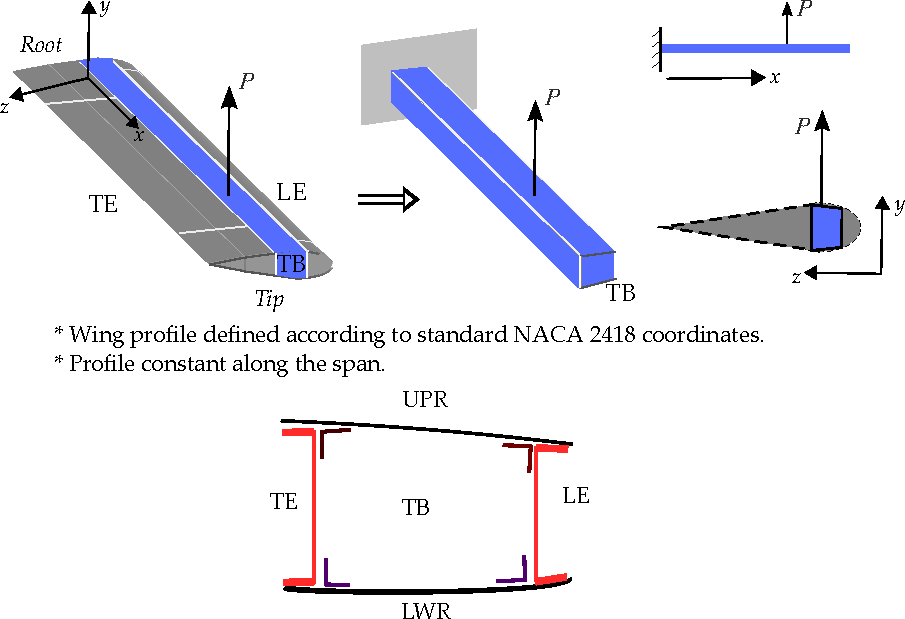
\includegraphics[width=\textwidth]{ASD2-DBT-Wing-5-revised-2018.pdf}
  \caption{Schematic of a typical wing torque box - NACA 2418 profile. (LE) - Leading edge, (TB) - Torque box, (TE) - trailing edge  - \textit{(Ian Farrow 2013)}.}
  \label{fig:ASD2-DBT-Wing-5-revised}
\end{figure}

\section{Description of wing torque box}

\begin{enumerate}
	\item Provide a brief description of component, basic design details, and functionality.
\end{enumerate}
%
\begin{quote} ...a representative CAD model of a generic torque box (TB) prototype is shown in Fig.~\ref{fig:wing-cad-model}. Key structural features are: 

\begin{itemize}
\item \textbf{Spars} Vertical elements running along the wingspan. They have the main function of carrying the shear force; 
\item \textbf{Stringers} Slender beams attached to the skin. They have the main function of carrying the axial force (thus balancing the wing bending moment) and stabilizing the skin against buckling; 
\item \textbf{Skin} Thin shell covering the wing. It has the main function of carrying the wing torsional moments and providing the aerodynamic shape; 
\item \textbf{Ribs} Elements located in the cross-section plane. They have the main function of maintaining the shape and redistributing the external loads.
\end{itemize}
%
Although several simplifications have been made (e.g.~absence of LE droop-nose and TE flap), the proposed structure contains sufficient detail for an initial FE analysis to capture the phenomena of interest. The CAD that has been prepared for this exercise is a reduced version of this wing torque box, containing only surfaces and curves (lines) to represent the main geometric features (see Fig.~\ref{fig:wing-cad-model-cleanup})...\end{quote}
%
\begin{figure}
  \begin{center}
  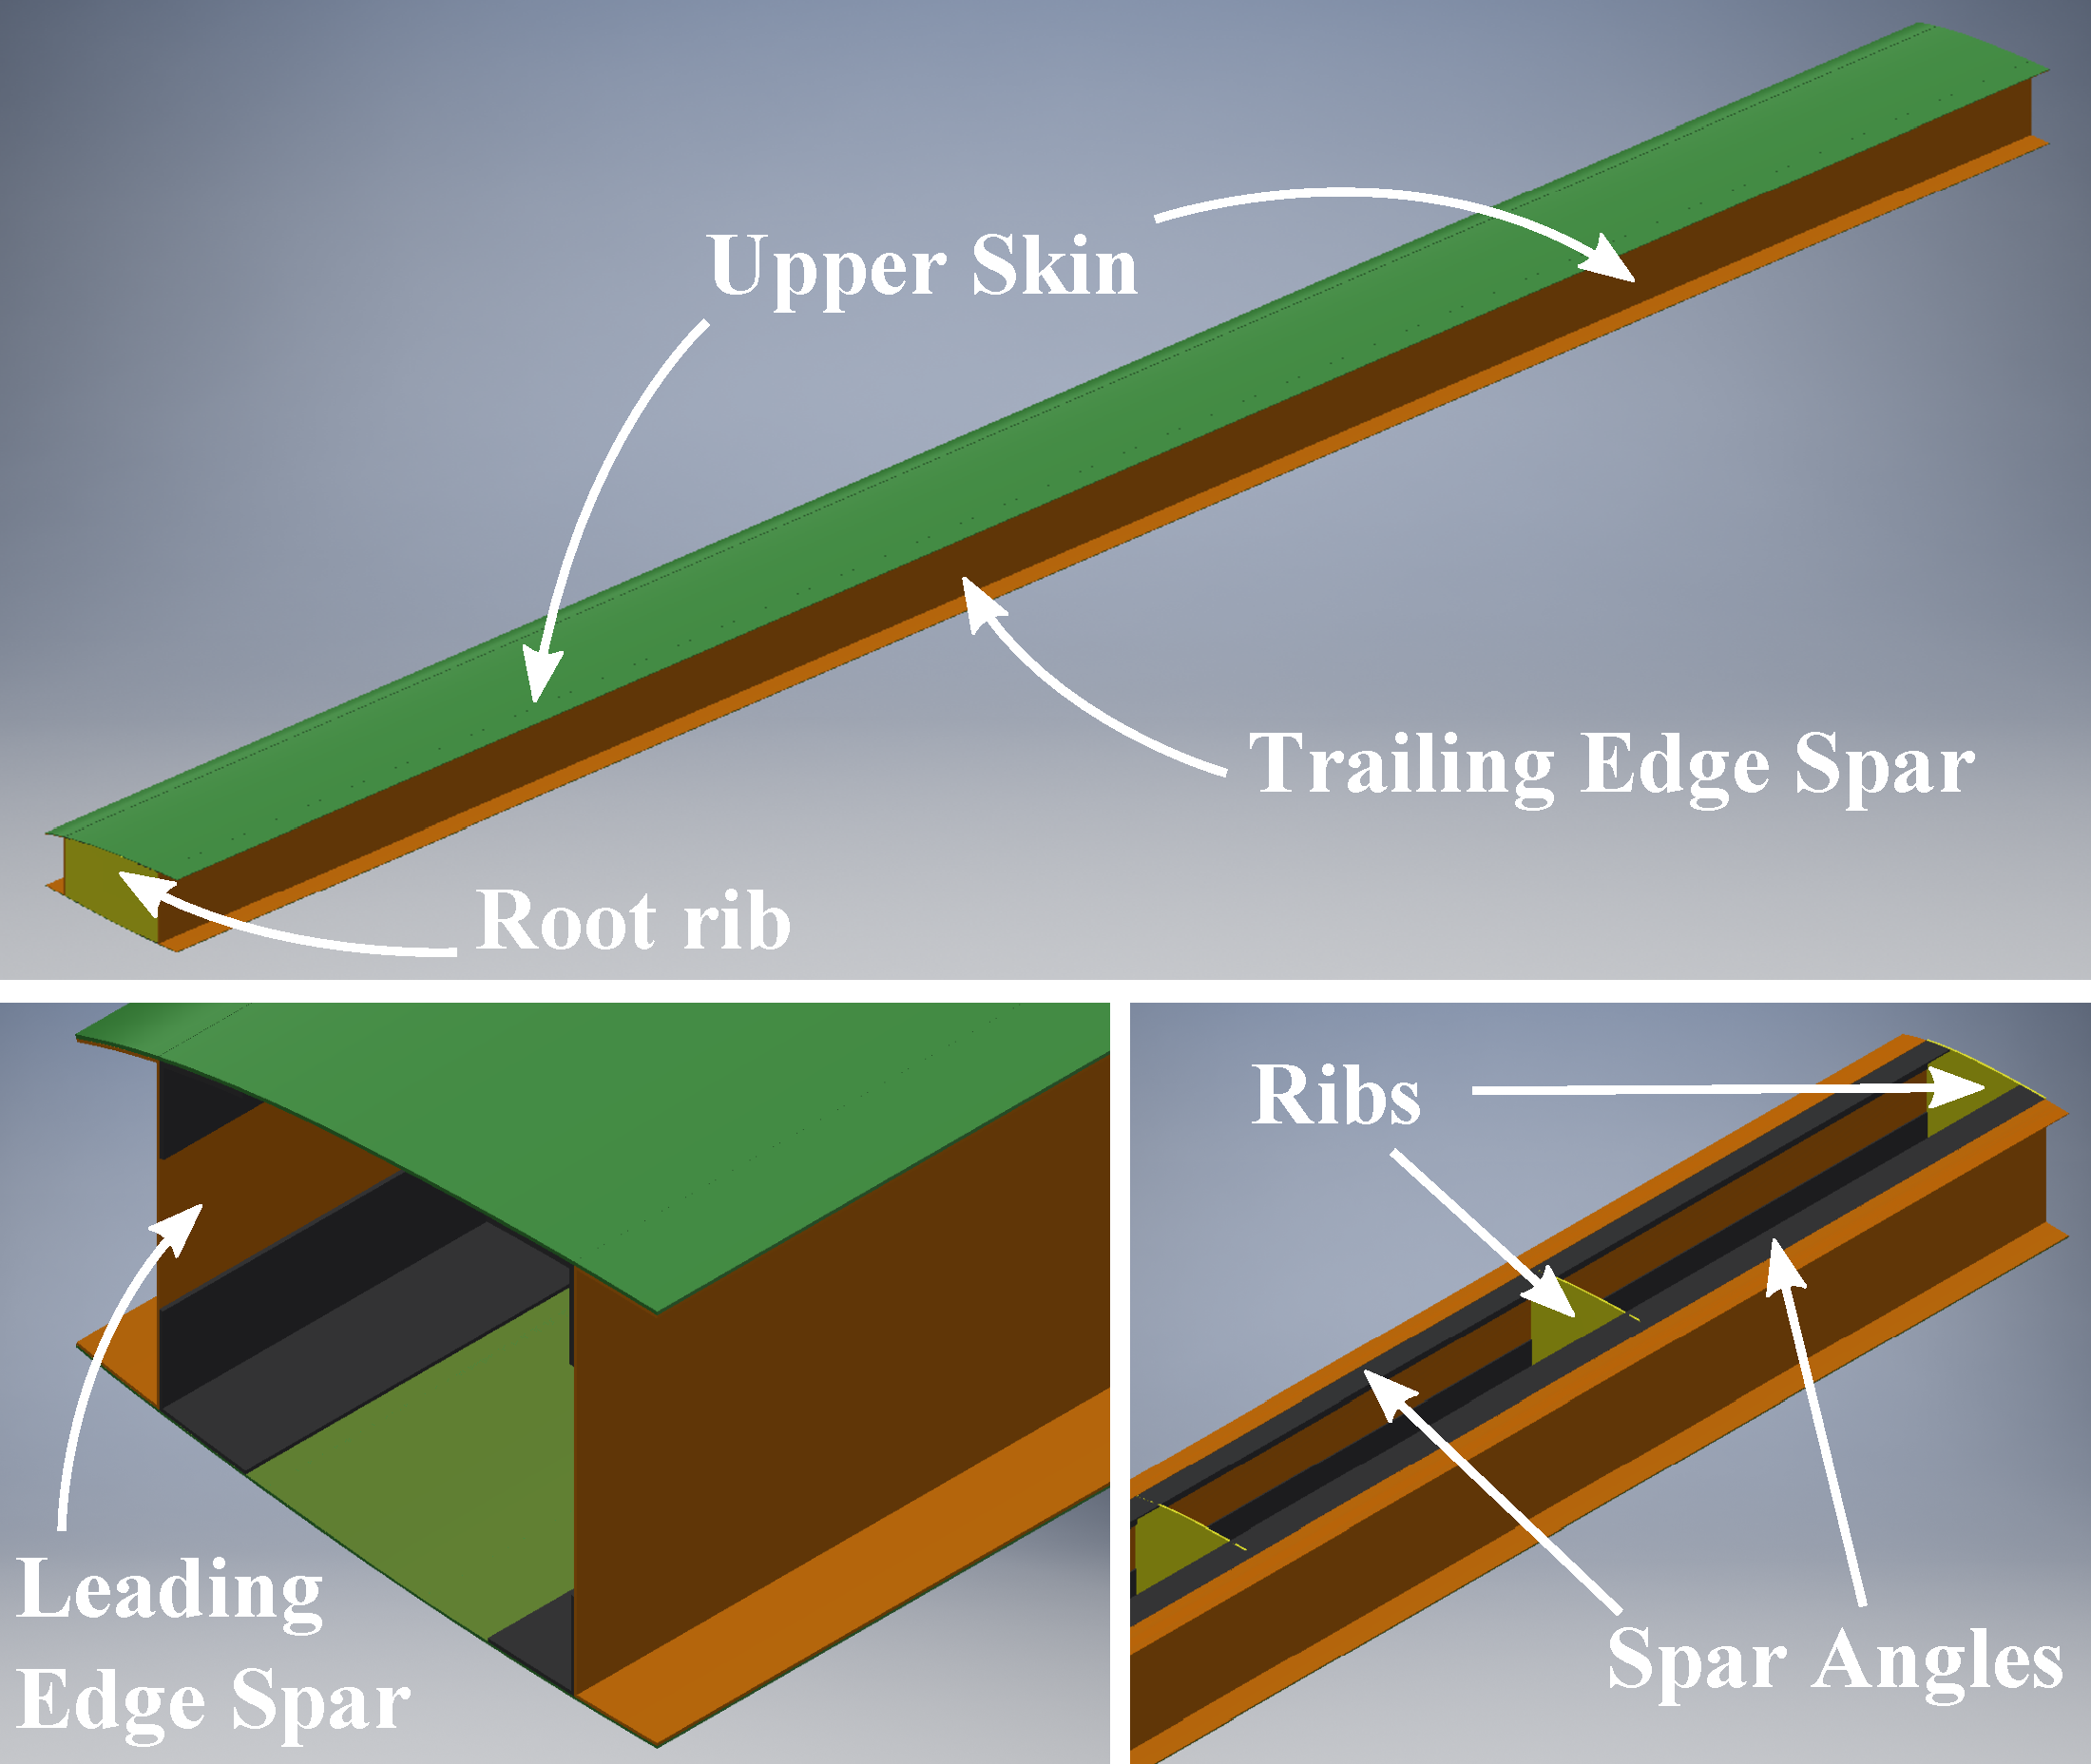
\includegraphics[width=\textwidth]{wing-cad-model-2018.pdf}
  \caption{Representative CAD model of torque wing box highlighting key structural features.}
  \label{fig:wing-cad-model}
  \end{center}
\end{figure}
%
\begin{figure}[t]
  \begin{center}
  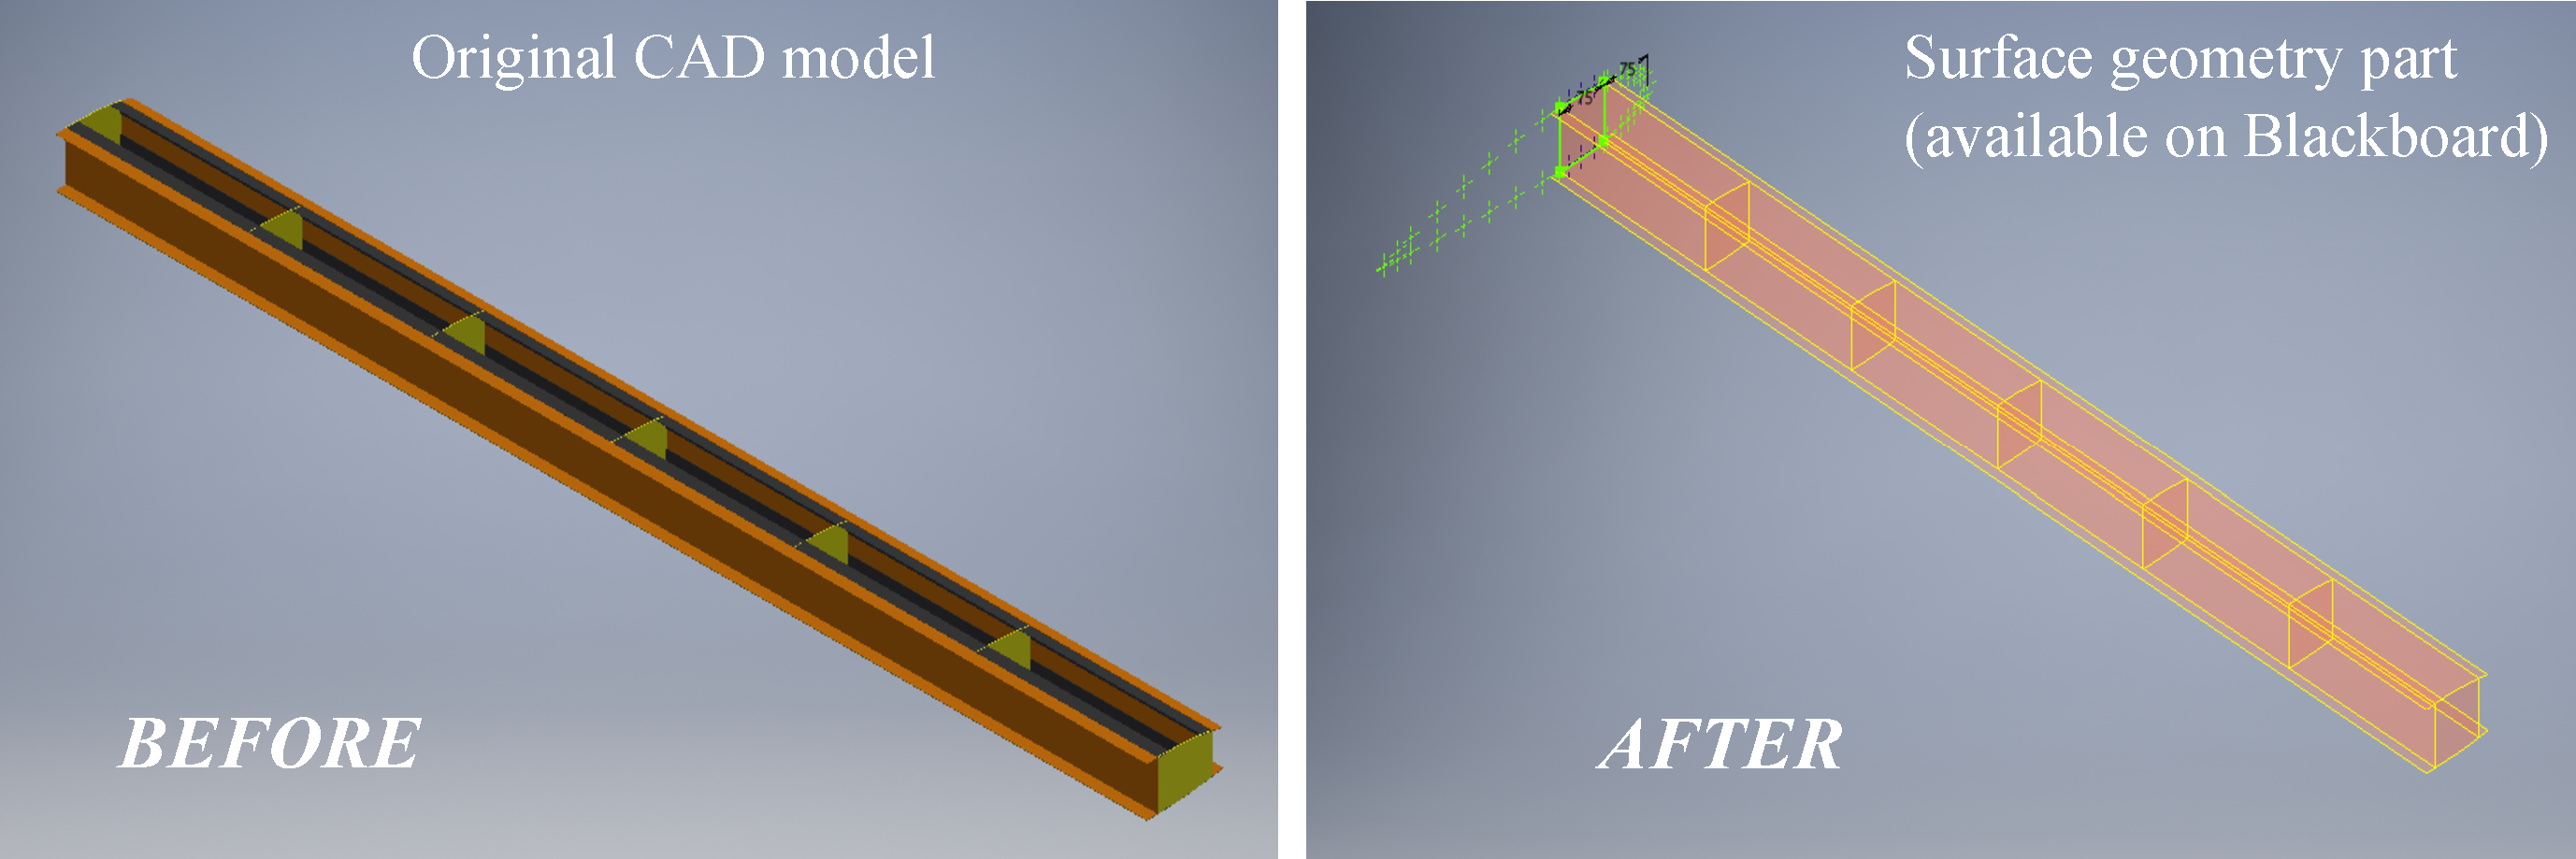
\includegraphics[width=1\textwidth]{wing-cad-model-cleanup.pdf}
  \caption{Final IGES file available on Blackboard after CAD clean-up and repair.}
  \label{fig:wing-cad-model-cleanup}
  \end{center}
\end{figure}

\subsection{Boundary and loading conditions} 
The torque box is idealised as a cantilever beam with an offset load, as illustrated in Fig. \ref{fig:ASD2-DBT-Wing-TB-Loading-Boundary}. Only one load case shall be considered, where the value of \mbox{$P = 1.0$ kN}. 
To best mimic the structural root attachments from AVDASI2, the following boundary conditions (BCs) are suggested:
\begin{description}
\item[1. Trailing Edge spar:] To represent the TE bending reaction joint plates, assign fully constrained boundary conditions at the TE, see Fig.~\ref{fig:ASD2-DBT-Wing-TB-Loading-Boundary}. 	
\item[2. Baseplate:] Entire wing root is constrained in the global $X$ (span-wise) direction. Note that this BC implies that all of the sections are active at the root.
\end{description}

\begin{figure}
    \centering
    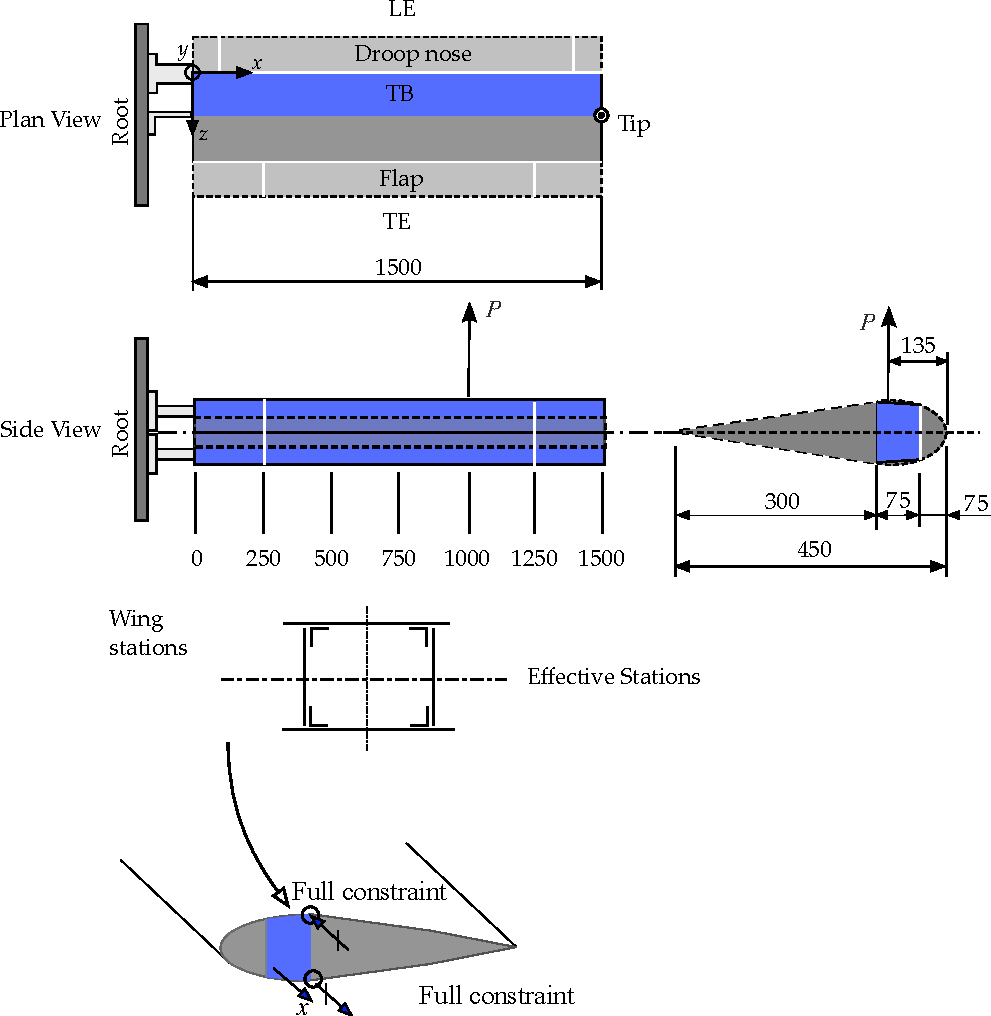
\includegraphics[width=.98\textwidth]{ASD2-DBT-Wing-TB-Loading-Boundary-2018}
    \caption{Schematic of boundary (restraint) and loading conditions applied to wing torque box \textit{(Ian Farrow 2013)}.}
  \label{fig:ASD2-DBT-Wing-TB-Loading-Boundary}
\end{figure}
%\begin{figure}
%    \centering
%    \includegraphics[scale=1.0]{ASD2-DBT-Wing-TB-Loading-Boundary-6}
%    \caption{Schematic of structural test arrangement of root fixture boundary conditions \textit{(Ian Farrow 2013)}.}
%  \label{fig:ASD2-DBT-Wing-TB-Loading-Boundary-2}
%\end{figure}
\clearpage
\subsection{Geometric properties of structural elements}

Table \ref{tab:wing-size} gives the dimensions of key structural elements of the torque box that should be employed in the sectional properties definition of the finite element model, as illustrated in Fig.~\ref{fig:wing-cad-model-view}.

\begin{figure}
    \begin{center}
    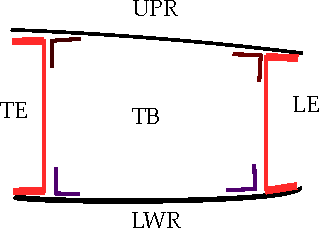
\includegraphics[scale=1.0]{wing-cad-model-view.pdf}
    \caption{Cross-section of the wing torque box showing key structural features: skin, stringers and spars.}
    \label{fig:wing-cad-model-view}
    \end{center}
\end{figure}

Spar cap angles are composed of L profiles cross-sectional areas. 

All structural elements are manufactured from the aerospace standard clad aluminium alloy 'Aluminium 2014a-T3'\footnote{Recall temper notation : T3 - Solution heat treated, cold worked and naturally aged}. Typical material properties for 2014 aluminium alloy are given in Table \ref{tab:wing-size}.  
%
\begin{table}[!h]
\centering
\caption{Dimensions and sizes of the wing and its structural elements.}
\label{tab:wing-size}
\begin{tabular}{llc}
\toprule
Element              & Thickness [mm]  &   Additional comments  \\    
\midrule
UPR skin             & 0.8         &  \\
LWR skin             & 0.5         &  \\
                     &             &  \\
LWR spar cap angle   & 0.9         &  All angles: L profile  \\
UPR spar cap angle   & 0.7         &  15 $\times$ 15 mm\\
                     &             &  \\
LE spar              & 0.5         &  \\
TE spar              & 0.5         &  \\
                     &             &  \\
Ribs                 & 1.0         &  \\
                     &             &  \\
%Span length          & 1500        &  \\
\midrule
\multicolumn{3}{c}{Material : Aluminium 2014a-T3}\\
\multicolumn{3}{c}{E = 73 GPa, $\nu$ = 0.3, $\rho$=2800 kg/m$^{3}$}\\
\multicolumn{3}{c}{Tensile and compressive allowable limit: 245 MPa}\\
\bottomrule
\end{tabular}
\end{table}

%
\chapter{Finite Element Model}\label{chap:fe-model}
\section{Pre-processing steps}Discuss very briefly the pre-processing steps:
\begin{enumerate}
    \item The IGE file which contains the torque box geometry was imported into PATRAN.The surfaces were then broken along the span into six equal sections. This allows the ribs to be created. The surfaces were broken down by the projection of the inboard edges onto 5 equally spaced planes.
    \item The unit system used in this model was millimetre for length and Newton for force.
    \item Material used in this model was Aluminium 2014a T3 with the properties as stated in table \ref{tab:wing-size}. The model used assumed an isotropic material which means the material is arranged in the same direction for the whole torque box model. Material decription is shown in figure \ref{fig:ex.1-bdf} labeled \textbf{4.}
    \item The skins of the box were assigned a 2D shell properties with varied thickness as indicated in table \ref{tab:wing-size}. This can also be seen in figure \ref{fig:ex.1-bdf} where \textbf{3.} shows different thickness for different shell properties. The spar angle supports were created using the 1D beam element properties with 2 different thickness for upper and lower skins. They also have different orientation for 4 corners. The properties of these beams is shown in figure \ref{fig:ex.1-bdf} where \textbf{1.} shows the beam dimension in mm. and \textbf{2.} shows beam's thickness.
    \item The conditions stated in figure \ref{fig:ASD2-DBT-Wing-TB-Loading-Boundary} means the conditioned applied is 
    \begin{itemize}
        \item fixed in all 6 degrees of freedom at the trailing edge spar.
        \item fixed in translational x direction for the rest of the wing.
        \begin{figure}[h]
            \centering
            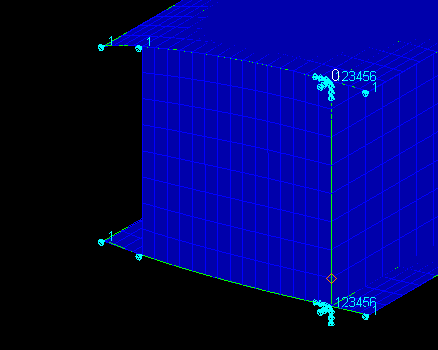
\includegraphics[width = .5\textwidth]{figures/boundary-condition.png}
            \caption{Boundary condition as applied in PATRAN}
            \label{fig:ex.1-bd}
        \end{figure}
    \end{itemize}
    PATRAN boundary condition constraints are shown in figure \ref{fig:ex.1-bd} .\\
    The load property  as listed in the .bdf file is labeled \textbf{5.} in figure \ref{fig:ex.1-bdf}. 

\begin{figure}[h]
    \centering
    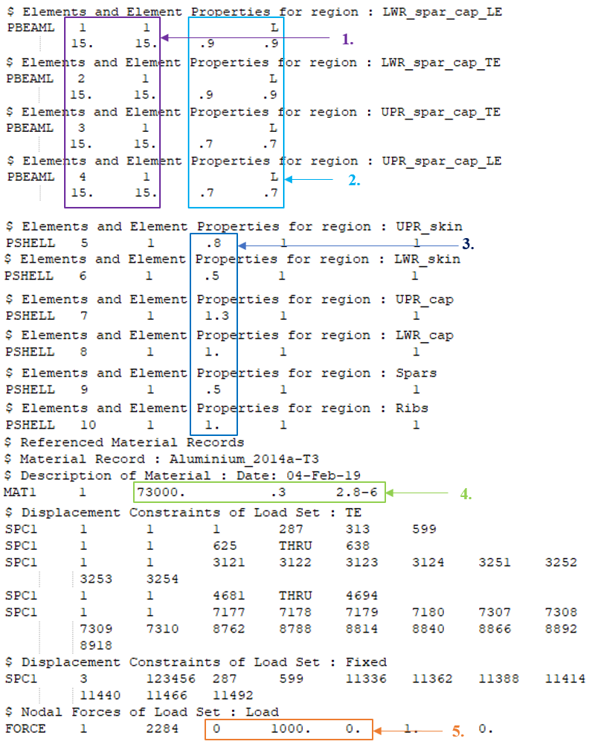
\includegraphics[width = .9\textwidth]{figures/bdf.png}
    \caption{Parts of the .bdf file which shows the shell and beam properties as well and boundary conditions and load.}
    \label{fig:ex.1-bdf}
\end{figure}

    \item (Mesh details - element types and formulations, number of elements, quality checks), see Table \ref{tab:summary-mesh}.
\end{enumerate}

\begin{table}[h]
\centering
\vspace{-2cm}
\caption{Summary of element types and aspect ratios assigned to each structural entity}
\label{tab:summary-mesh}	
\begin{tabular}{lccccc}
\toprule
Part               & \multicolumn{4}{c}{Total No. of elements}   & Element      \\
\cmidrule{2-5}     &  CBAR & CBEAM  & CQUAD4  & CTRIA3           &   size (AR)  \\
\midrule
UPR/LWR Skin       &   -    &  -      & 6900        &  -                &       2       \\
TE/LE Spar webs    &    -   &   -     &  2400       &     -             &        1.075      \\
TE/LE Angle caps   &  -     &   600     &    -     &    -              &        N/A      \\
Ribs               &   -    &     -   &  840       &        -          &           2   \\
\midrule
Total              &    -   &    600    &     10140    &       -           &              \\
\bottomrule
\end{tabular}
\end{table}

\chapter{Analytical Wing Sizing Calculations}\label{chap:hand-calcs}
\section{Initial wing sizing calculations}
\begin{enumerate}
	\item State all key assumptions, equations and simplifications. 
	\item Include an annotated sketch of the equivalent torque box and boom idealisation.
	\item You may tabulate the results directly from a working excel spreadsheet or Matlab script. However, place key calculations in the Appendix not in the main body of text. 
\end{enumerate}

\begin{enumerate}
    \item Key assumptions,
    \begin{itemize}
        \item The structure is modelled using the thin-wall assumptions for semi-monocoque structure.
        \item Also, assume the skin carries only shear when buckled.
        \item  Assume only the skin area get stabilised by the corner flanges when estimate the effective end load.
        \item Reduce the stabilised web and angle blade areas by one third to avoid overestimating the second moment of area contribution of the spar web and angle blade to the box.
    \end{itemize}
\end{enumerate}

\chapter{Results of Finite Element Model}\label{chap:results}
\section{Results from Exercise \#1}
\begin{enumerate}
	\item Tabular results and clear figures of appropriate load case, see Table \ref{tab:summary-results}.
\end{enumerate}

\begin{table}[h]
\centering
\caption{Summary of stress and deflection results as obtained from MSC Nastran linear static model.}
\label{tab:summary-results}
\begin{tabular}{lccc}
  \toprule
  Component                           & Value & Location & Fig. No.   \\
  \midrule
  Max. displacement                   &  20.2 mm. &     Node 4679     &     \ref{fig:max-displacement}       \\
  \midrule
  Max. von Mises stress (shell)       &  132 Nmm\textsuperscript{-2}& Node 313  &    \ref{fig:max-von-mosses}        \\
  \midrule
  Max. shear stress (shell)           &  71.2 Nmm\textsuperscript{-2} & Node 313 &   \ref{fig:max-shear}        \\
  \midrule
  Max. combined axial and             &  208 Nmm\textsuperscript{-2} & Node 313 &   \ref{fig:combined-beam}         \\
  bending stress (beam)               &       &          &            \\
  \midrule
  Mass of the wing torque box         &  1.537 kg &    n/a   &   n/a      \\  \bottomrule
\end{tabular}\end{table}
\begin{figure}[h]
    %\begin{minipage}{.5\textwidth}
    \centering
    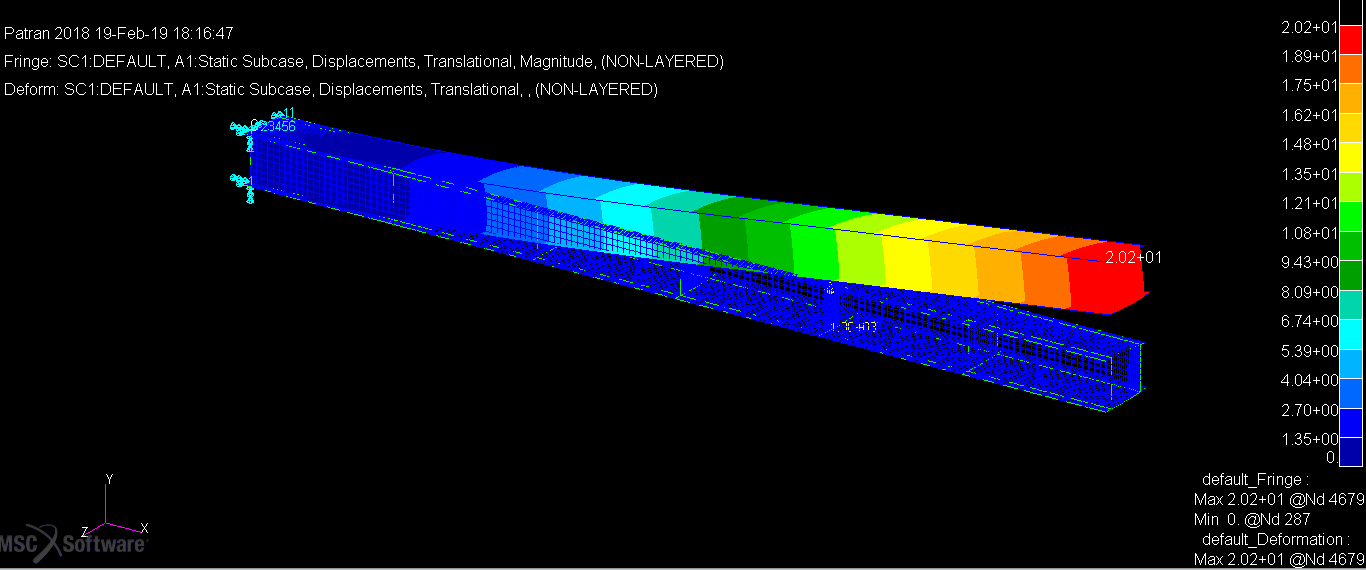
\includegraphics[width = .8\textwidth]{figures/one-displacement-2.png}
    \caption{Max. Displacement of the whole torque box}
    \label{fig:max-displacement}
    %\end{minipage}%
\end{figure}
\begin{figure}[h]
    %\begin{minipage}{.5\textwidth}
    \centering
    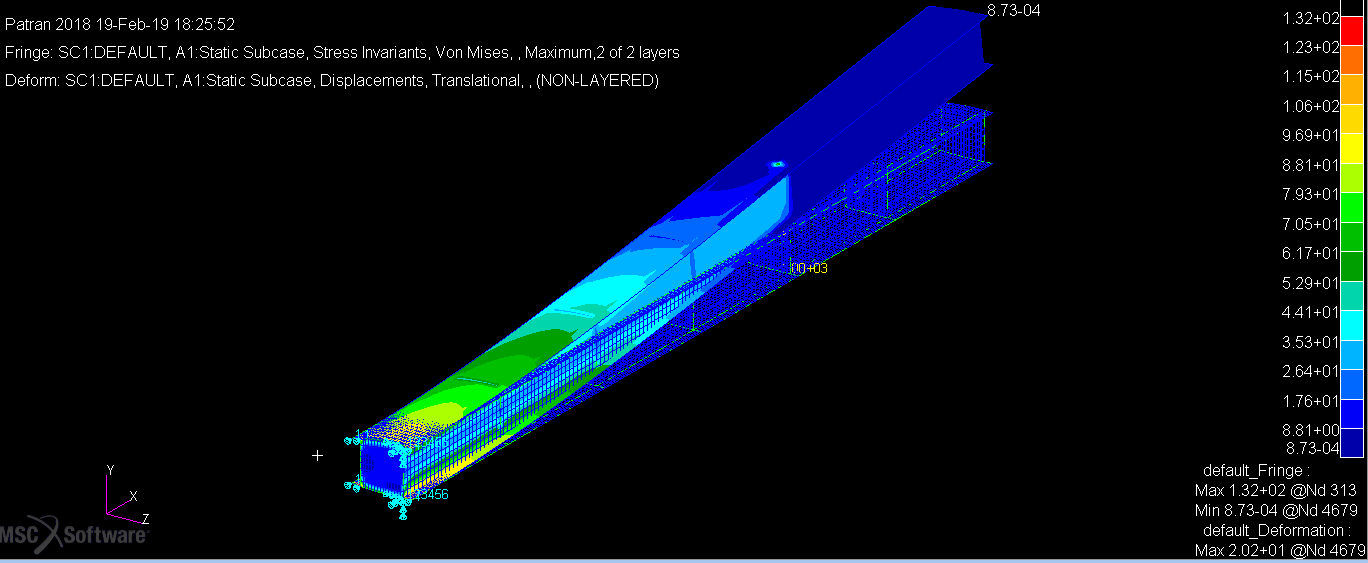
\includegraphics[width = .8\textwidth]{figures/one-von-misses.png}
    \caption{Max. von Misses stress}
    \label{fig:max-von-mosses}
    %\end{minipage}
\end{figure}
\begin{figure}[h]
    %\begin{minipage}{.5\textwidth}
    \centering
    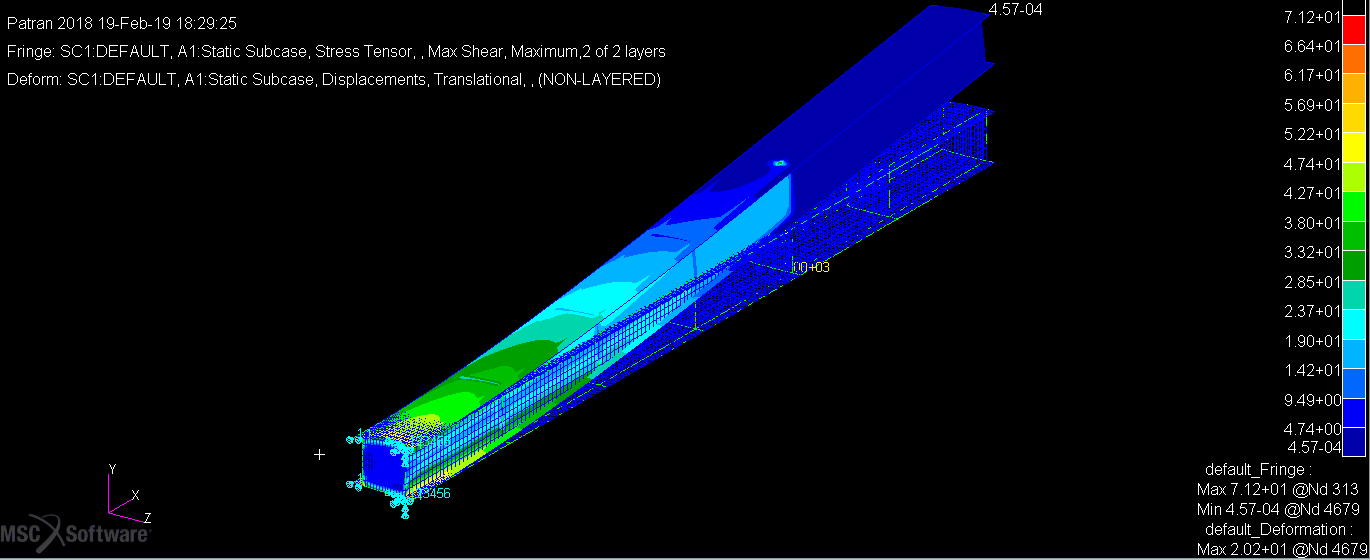
\includegraphics[width = .8\textwidth]{figures/one-max-shear.png}
    \caption{Max. shear stress}
    \label{fig:max-shear}
    %\end{minipage}%
\end{figure}
\begin{figure}[h]
    %\begin{minipage}{.5\textwidth}
    \centering
    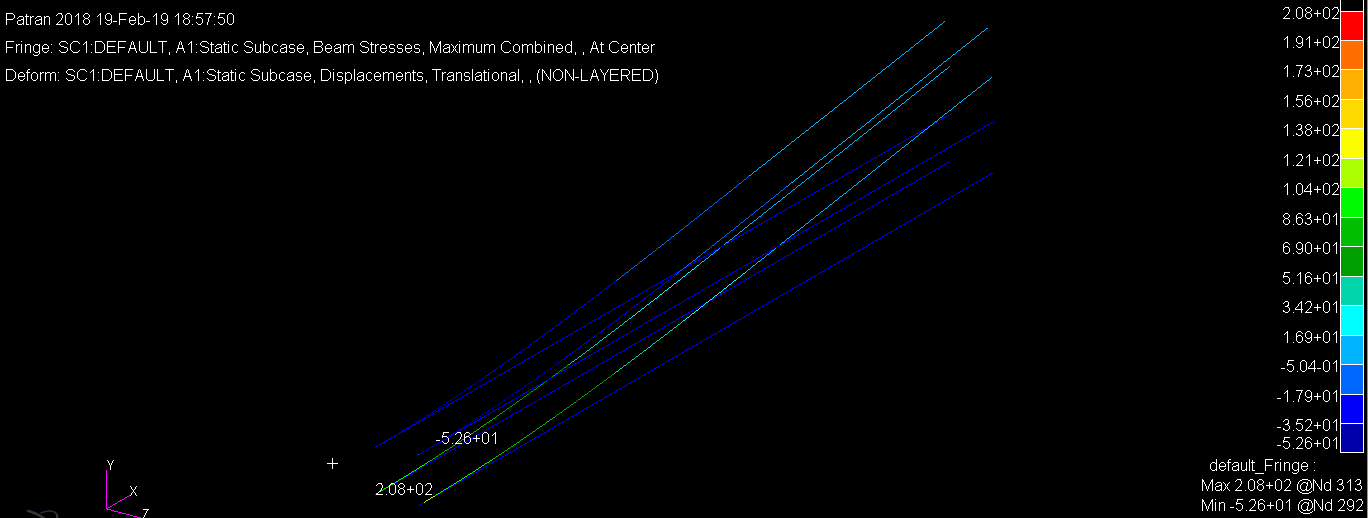
\includegraphics[width = .8\textwidth]{figures/one-combined-beam-stress.png}
    \caption{Max. combined axial and bending stress in beam elements.}
    \label{fig:combined-beam}
    %\end{minipage}
\end{figure}

\section{Verification against Analytical Solutions}
\begin{enumerate}
	\item Compare and discuss analytical and FE reserve factors.
\end{enumerate}

\begin{center}
	\begin{tabular}{ccccccc}
		\toprule
		            & UPR TE   & UPR skin & TE spar  & LWR skin & LWR TE  & Max tip  \\
		            & col. bkl.& buckling & buckling & tension  & tension & deflect. \\
		\midrule
		FE          &  RF val  &  RF val  &  RF val  &  RF val  & RF val  &  (mm)   \\
		\midrule
		Analytical  &  RF val  &  RF val  &  RF val  &  RF val  & RF val  &  (mm)   \\
		\bottomrule
	\end{tabular}
\end{center}

\section{Discussion of Results}
\begin{enumerate}
	\item Use engineering judgement to comment on the structural integrity of the wing torque box based on your stress results and stress allowable for the aluminium material. 
	\item Does the FE model fully capture the structural behaviour of the wing torque-box under the loading specified?
	\item What are the limitations of the current 'linear static model'?
\end{enumerate}	

\section{Improvements to FE Design - Inspection hole analysis}
\begin{enumerate}
	\item Discuss the geometry creation, namely how to partition the geometry and create the inspection holes cuts.
	\item Present images of the von Mises stress field on the lower skin without and with inspection holes. Discuss differences.
	\item Calculate the stress concentration factor on each inspection hole. Present results in a table.
	\item Present a graph showing the distribution of stress in a chord-wise direction on an inspection hole. Discuss stress concentration around a hole.
	\item Discuss the re-distribution of stress after including the inspection holes. How has the stress been distributed in the skin/booms?
\end{enumerate}

\begin{enumerate}
    \item The geometry of the inspection holes were created by the following steps:
    \begin{itemize}
        \item Six planes were created in the middle of the six bays with the vector [0,1,0] as the reference vector. A circle with radius of 15mm was then created on each plane. Each lower skin panel was then being sectioned as shown in figure \ref{fig:ex.3-surface}
        \begin{figure}[h]
            \centering
            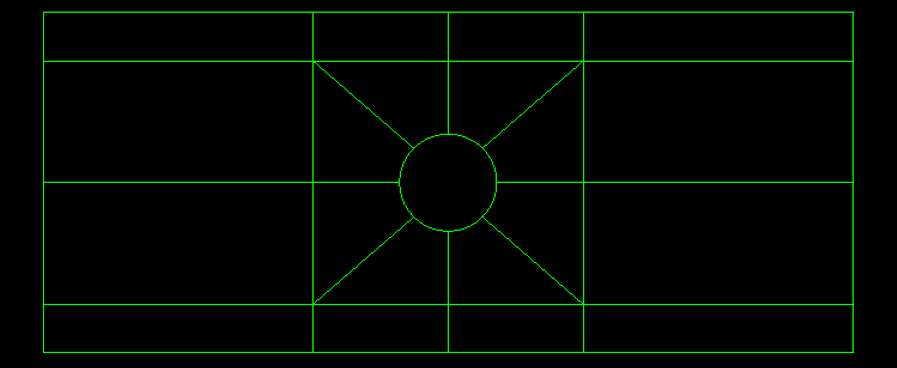
\includegraphics[width = .7\textwidth]{figures/LWR-surface.png}
            \caption{Surface break of a section from a lower skin panel.}
            \label{fig:ex.3-surface}
        \end{figure}
        The surfaces were created  in this panel apart from inside the circle; this created a hole.
    \end{itemize}
    \item Figure \ref{fig:von-misses-holes} and \ref{fig:von-misses-w/o-holes} show the von Misses stress distribution along the lower skin in the case with and without the inspection holes.
    \begin{figure}[h]
        \centering
        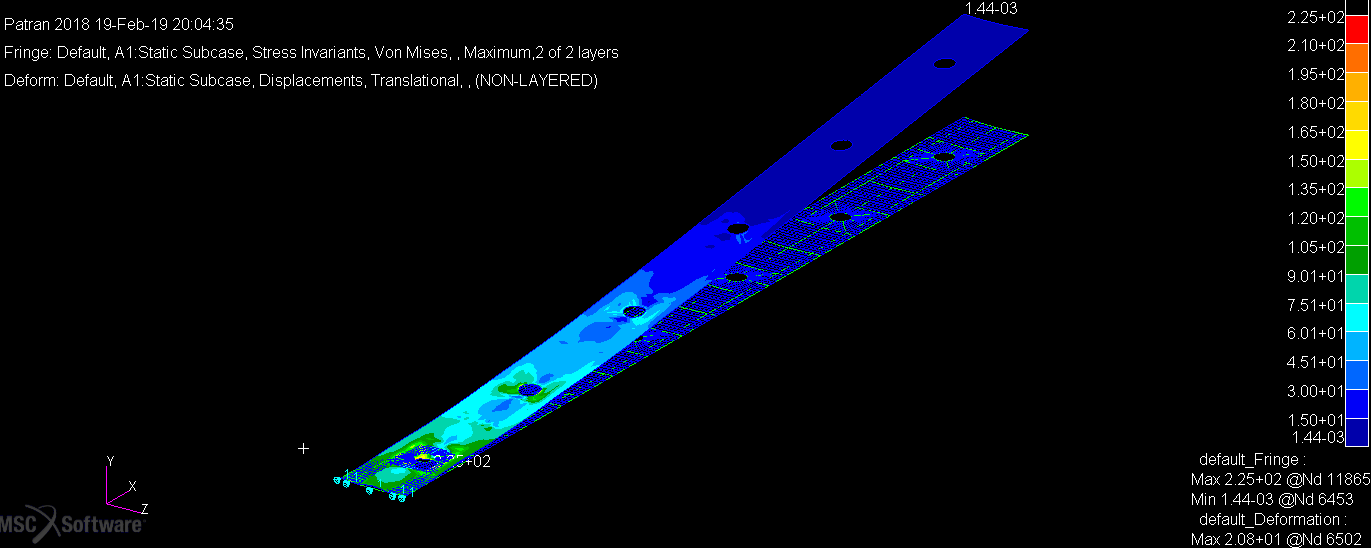
\includegraphics[width = .8\textwidth]{figures/stress-distribution.png}
        \caption{von Misses stress distribution in the lower skin with inspection holes.}
        \label{fig:von-misses-holes}
    \end{figure}
    \begin{figure}[h]
        \centering
        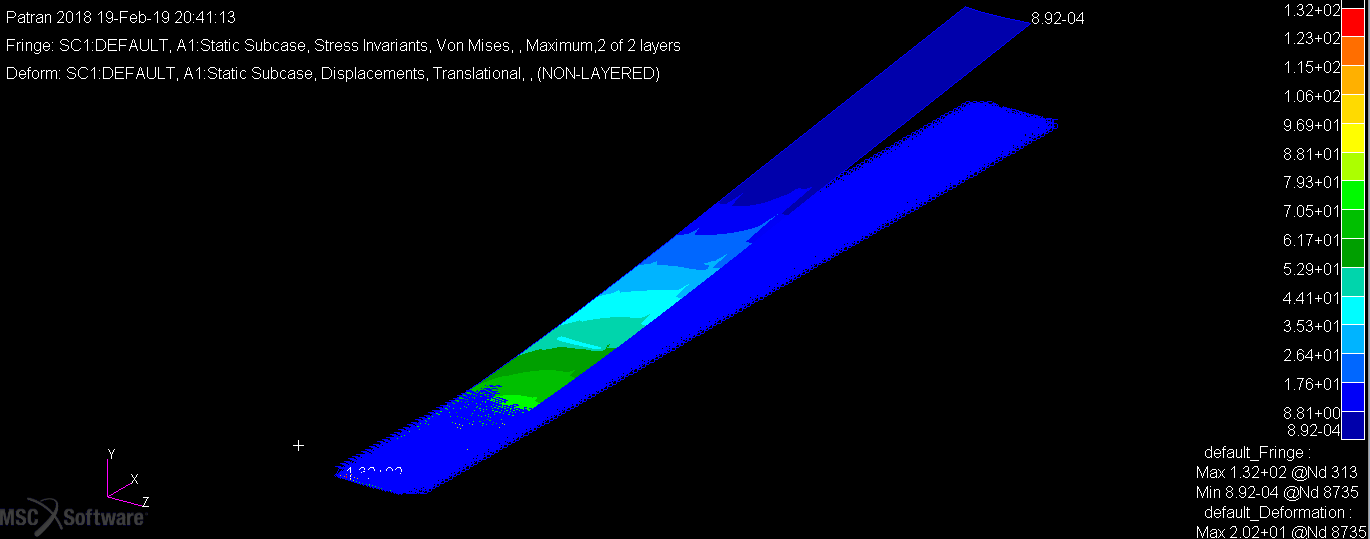
\includegraphics[width = .8\textwidth]{figures/one-LWR-skin-von-misses.png}
        \caption{von Misses stress distribution in the lower skin without inspection holes.}
        \label{fig:von-misses-w/o-holes}
    \end{figure}
\begin{figure}[!hbt]
    \begin{minipage}{.5\textwidth}
    \centering
    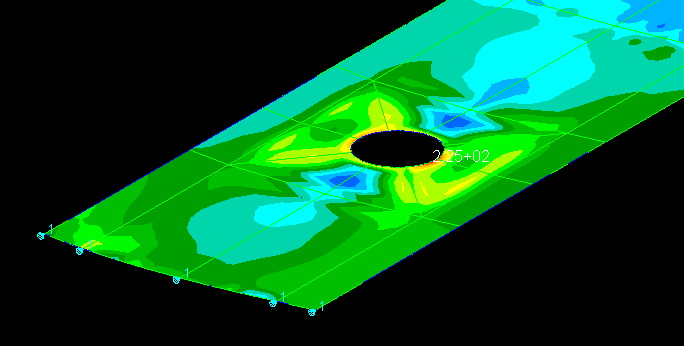
\includegraphics[width = .92\textwidth]{figures/three.png}
    \caption{A closer look at figure \ref{fig:von-misses-holes}}
    \label{fig:von-misses-holes-zoom}
    \end{minipage}%
    \begin{minipage}{.5\textwidth}
    \centering
    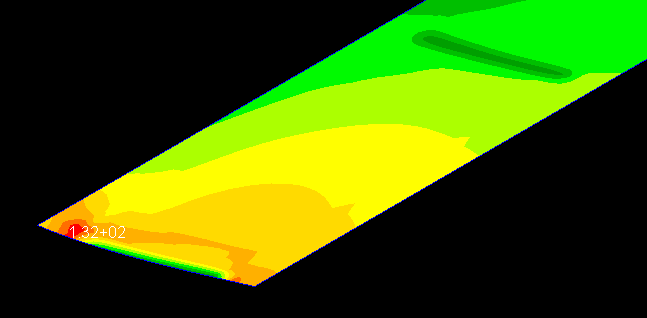
\includegraphics[width = .95\textwidth]{figures/one.png}
    \caption{A closer look at figure \ref{fig:von-misses-w/o-holes}}
    \label{fig:von-misses-w/o-holes-zoom}
    \end{minipage}
\end{figure}
    \textbf{DISCUSS DIFFERENCES}
    \item Table \ref{tab:stress-conc-factor} shows stress concentration factor in each inspection hole. The table which shows calculation for this can be found in appendix \textbf{APPENDIX IT}
    \item Figure \ref{fig:stress-along-chord-hole} and figure \ref{fig:stress-along-chord} show the stress distribution in a chord-wise direction. Figure \ref{fig:stress-along-chord-hole} shows the distribution on an inspection hole while figure \ref{fig:stress-along-chord} shows the one without.
\end{enumerate}

\begin{table}[h]
    \centering
    \begin{tabular}{l c}
    \toprule
      Hole   &  Stress concentration factor\\
     \midrule
      1   & 2.34\\
      2 &   3.12\\
      3 &   2.62\\
      4 &   2.74\\
      5 &   5.47\\
      6 &   1.72\\
      \bottomrule
    \end{tabular}
    \caption{Stress concentration factor in each inspection hole.}
    \label{tab:stress-conc-factor}
\end{table}

\begin{figure}[h]
    \centering
    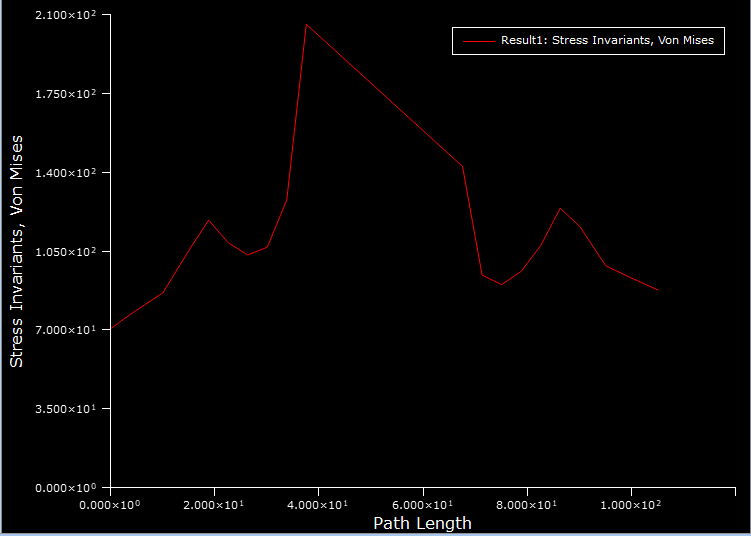
\includegraphics[width = .8\textwidth]{figures/Path-length.png}
    \caption{Distribution of stress along the chord-wise direction with an inspection hole.}
    \label{fig:stress-along-chord-hole}
\end{figure}

\begin{figure}[h]
    \centering
    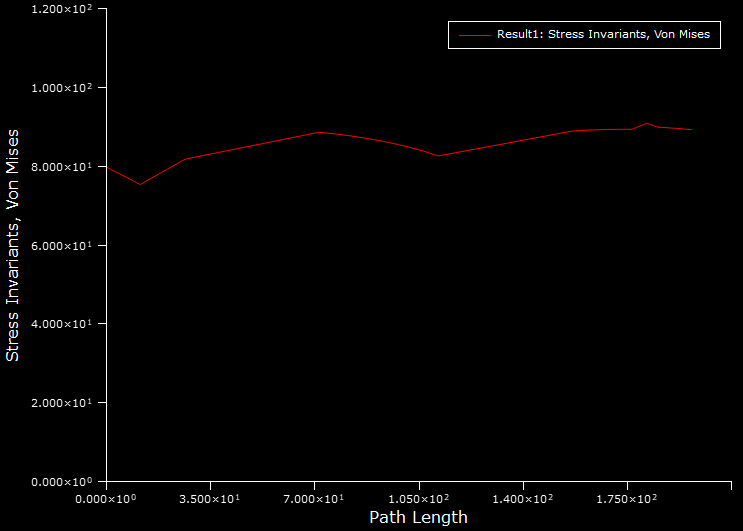
\includegraphics[width = .8\textwidth]{figures/Path-length-one.png}
    \caption{Distribution of stress along the chord-wise direction.}
    \label{fig:stress-along-chord}
\end{figure}



\chapter{Conclusions and Future Work}

\bibliographystyle{unsrt} % Title is link if provided
\bibliography{bibliography} % adjust this to fit your BibTex file

%: ----------------------- appendices ------------------------
\appendix

\chapter{MSC Nastran .bdf file}\label{chap:a}
\begin{enumerate}
	\item Copy of \underline{\textbf{truncated}} .bdf file from Exercise \#1.
\end{enumerate}

\chapter{Analytical Calculations}\label{chap:b}

% Backmatter

\pagestyle{empty}
\newgeometry{innermargin=1in,top=1.25in,bottom=1.25in}
\vspace*{17.5cm}
\begin{minipage}[b]{14cm}
          \begin{tabular}{l}
          
\includegraphics[width=6.0cm]{UoB-logo-black.pdf}\\
            \Large{\url{www.bristol.ac.uk/engineering/}}\\
                \large Department of Aerospace Engineering \\
                \large University of Bristol\\
                \large Queen's Building \\
                \large University Walk\\
                \large Bristol, BS8 1TR \\
                \large United Kingdom\\
            \hspace*{-0.2cm}\large \begin{tabular}{l l l}
               Tel:& \quad   &(+44) (0) 117 33 15311\\
               Fax:& \quad   &(+44) (0) 117 954 5666\\
%\large Email: & \quad & \href{mailto:antonio.melro@bristol.ac.uk}{antonio.melro@bristol.ac.uk}\\
            \end{tabular}\\         
            \\
            \\
          \end{tabular}
        \end{minipage}
\restoregeometry
\end{document}

\end{document}
%~~~~~~~~~~~~~~~~~~~~~~~~~~~~~~~~~~~~~~~~~~~~~~~~~~~~~~~~~~~~~
\end{document}  % End of document (closes \begin{document} command).
%~~~~~~~~~~~~~~~~~~~~~~~~~~~~~~~~~~~~~~~~~~~~~~~~~~~~~~~~~~~~~
